\documentclass[11pt,a4paper]{article}
\usepackage[utf8]{inputenc}
\usepackage[spanish]{babel}
\usepackage{biblatex}
\usepackage{amssymb, amsmath, amsbsy}
\usepackage{graphicx}
\usepackage{makeidx}
\usepackage{color,xcolor}
\usepackage[left=2cm,right=2cm,top=2cm,bottom=2cm]{geometry}
\usepackage[linkcolor=black,colorlinks=true,urlcolor=blue]{hyperref}
\usepackage{xcolor}
\usepackage{fancyhdr}
\usepackage{float}
\usepackage{subfigure}
\renewcommand{\baselinestretch}{1.5}
\addbibresource{bib.bib}
\setlength{\parindent}{0em}
\bibliography{bib}

\begin{document}

\thispagestyle{empty}
\begin{center}

\includegraphics[width=10cm]{logo udesa.PNG}
\end{center}


	\begin{center}
	\LARGE
	Herramientas Computaciones para Investigación
\\			\vspace{1cm}
\hrule
	\vspace{0.5cm}
	\LARGE
 Tema 2 - QGIS
\\		
		\vspace{0.5cm}
		\hrule
				\vspace{1cm}
	\large

	\vspace{2.5cm}
	\large
		Alumnos:\\
	\large
	Elard Amaya, Francisco Guerrero
	
	
	\vspace{1.3cm}
	\normalsize	
	Profesora:\\

	\normalsize
	Amelia Gibbons
	
	\vspace{1.3cm}
	\today
	\end{center}

	
\clearpage
\section*{Parte 1 - Datos de Airbnb}

En la primera parte del trabajo, empleamos los datos de Airbnb de la ciudad de Chicago para el periodo 2008-2015. Esta base de datos contiene información sobre una serie de indicadores socio-económicos e indicadores del alcance de Airbnb para 77 comunidades de la ciudad. Hemos generado tres indicadores partiendo de la información de esta base: Ocurrencia de crímenes cada cien mil habitantes, tasa de aceptación de Airbnb e índice de Hardship. Para estos indicadores hemos empleado mapas coropléticos, los cuales nos permiten identificar el nivel de variabilidad de estos indicadores entre las 77 comunidades de Chicago.
\\ 
Con el mapa de ocurrencia de crímenes (Figura 1) buscamos identificar las zonas de mayor actividad criminal, saber si siguen algún patrón de agrupación, lo cual podría hacer estas zonas menos atrayentes para el servicio de hospedaje. Por otro lado, la tasa de aceptación de Airbnb(Figura 2) nos permite conocer cuáles son las zonas más demandadas y en consecuencia las zonas más valorizadas en el servicio de hospedaje por algunas cualidades particulares. Finalmente, el índice de Hardship(Figura 3) es una medida de bienestar, mientras este índice se encuentra más cercano al cero indica que el individuo se encuentra en una posición de bienestar superlativa, por el contrario, mientras más cercano esta del cien el individuo se encuentra en una posición más vulnerable. El índice de Hardship nos permite identificar las comunidades en las cuales habitan personas con mayor/menor bienestar, lo cual también se puede reflejar en la calidad de servicios e infraestructura que ofrece la comunidad y en consecuencia una aproximación a las zonas con mayor comodidad para el servicio de hospedaje. 

\begin{figure}[!h]
    \centering
    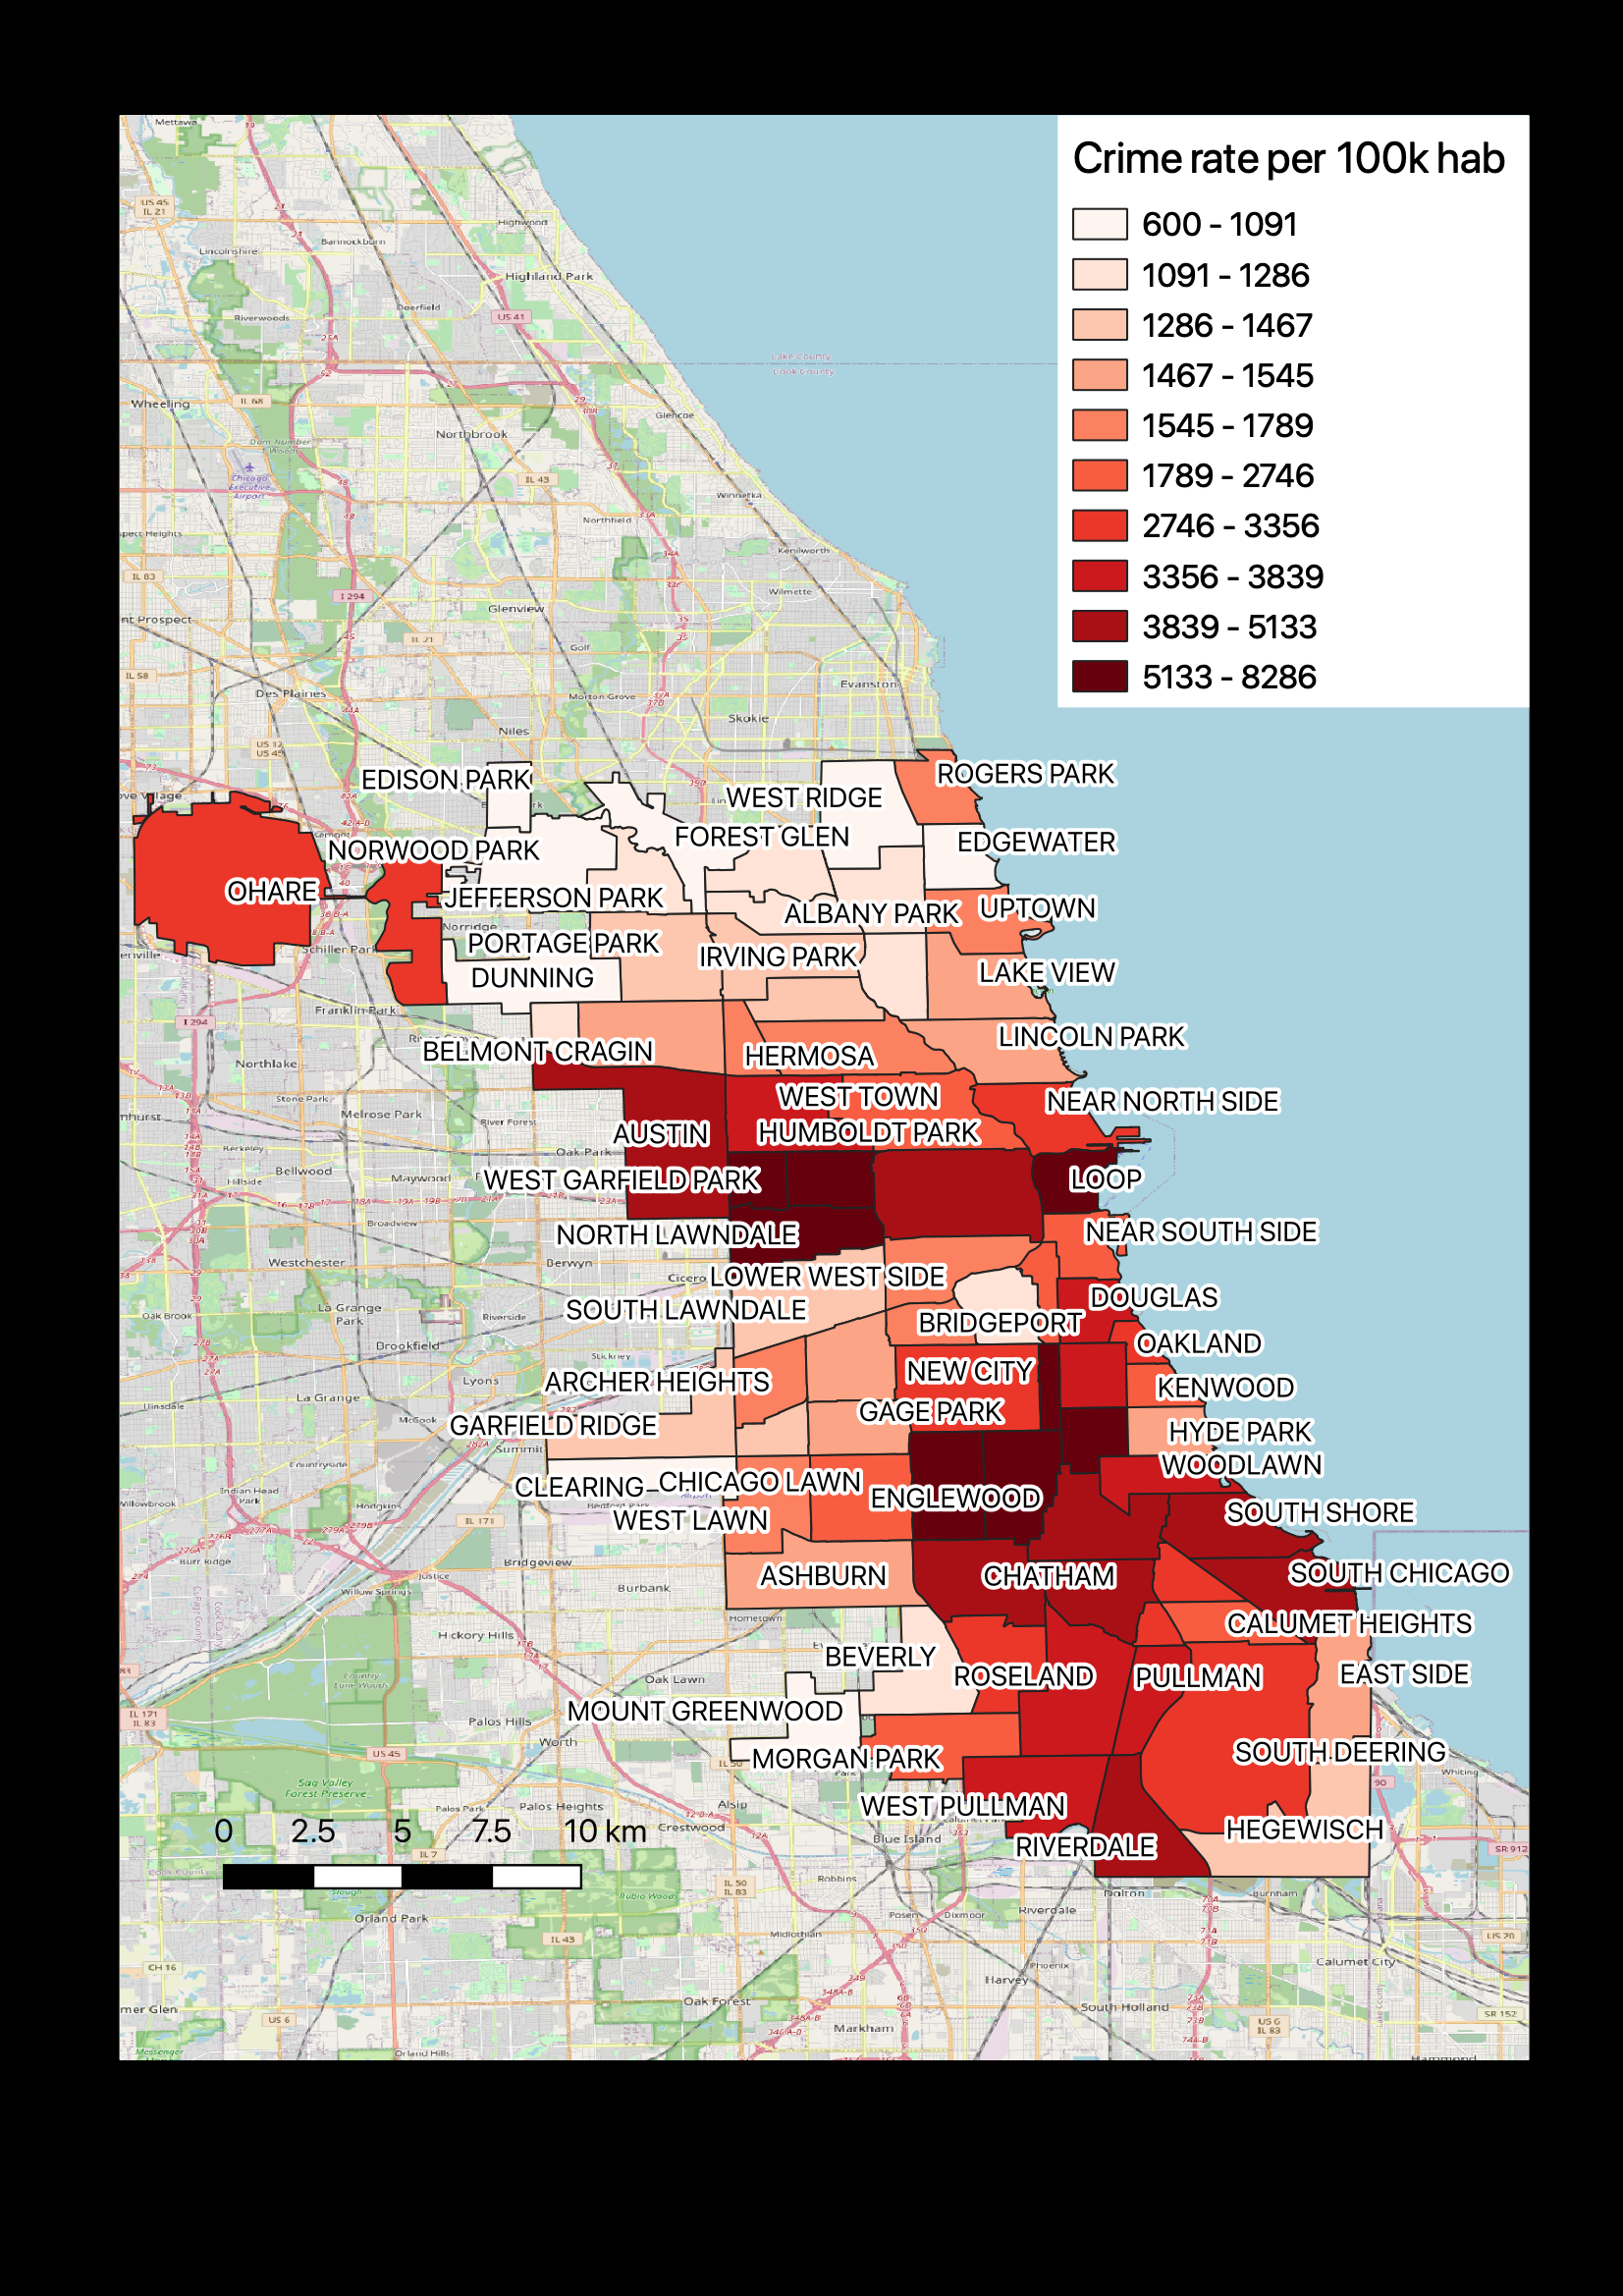
\includegraphics[width=7cm]{Crime-rate.png}
   \caption{Ocurrencia de crimen cada 100mil habitantes}
    \label{fig:my_label}
\end{figure}

\begin{figure}[!h]
    \centering
    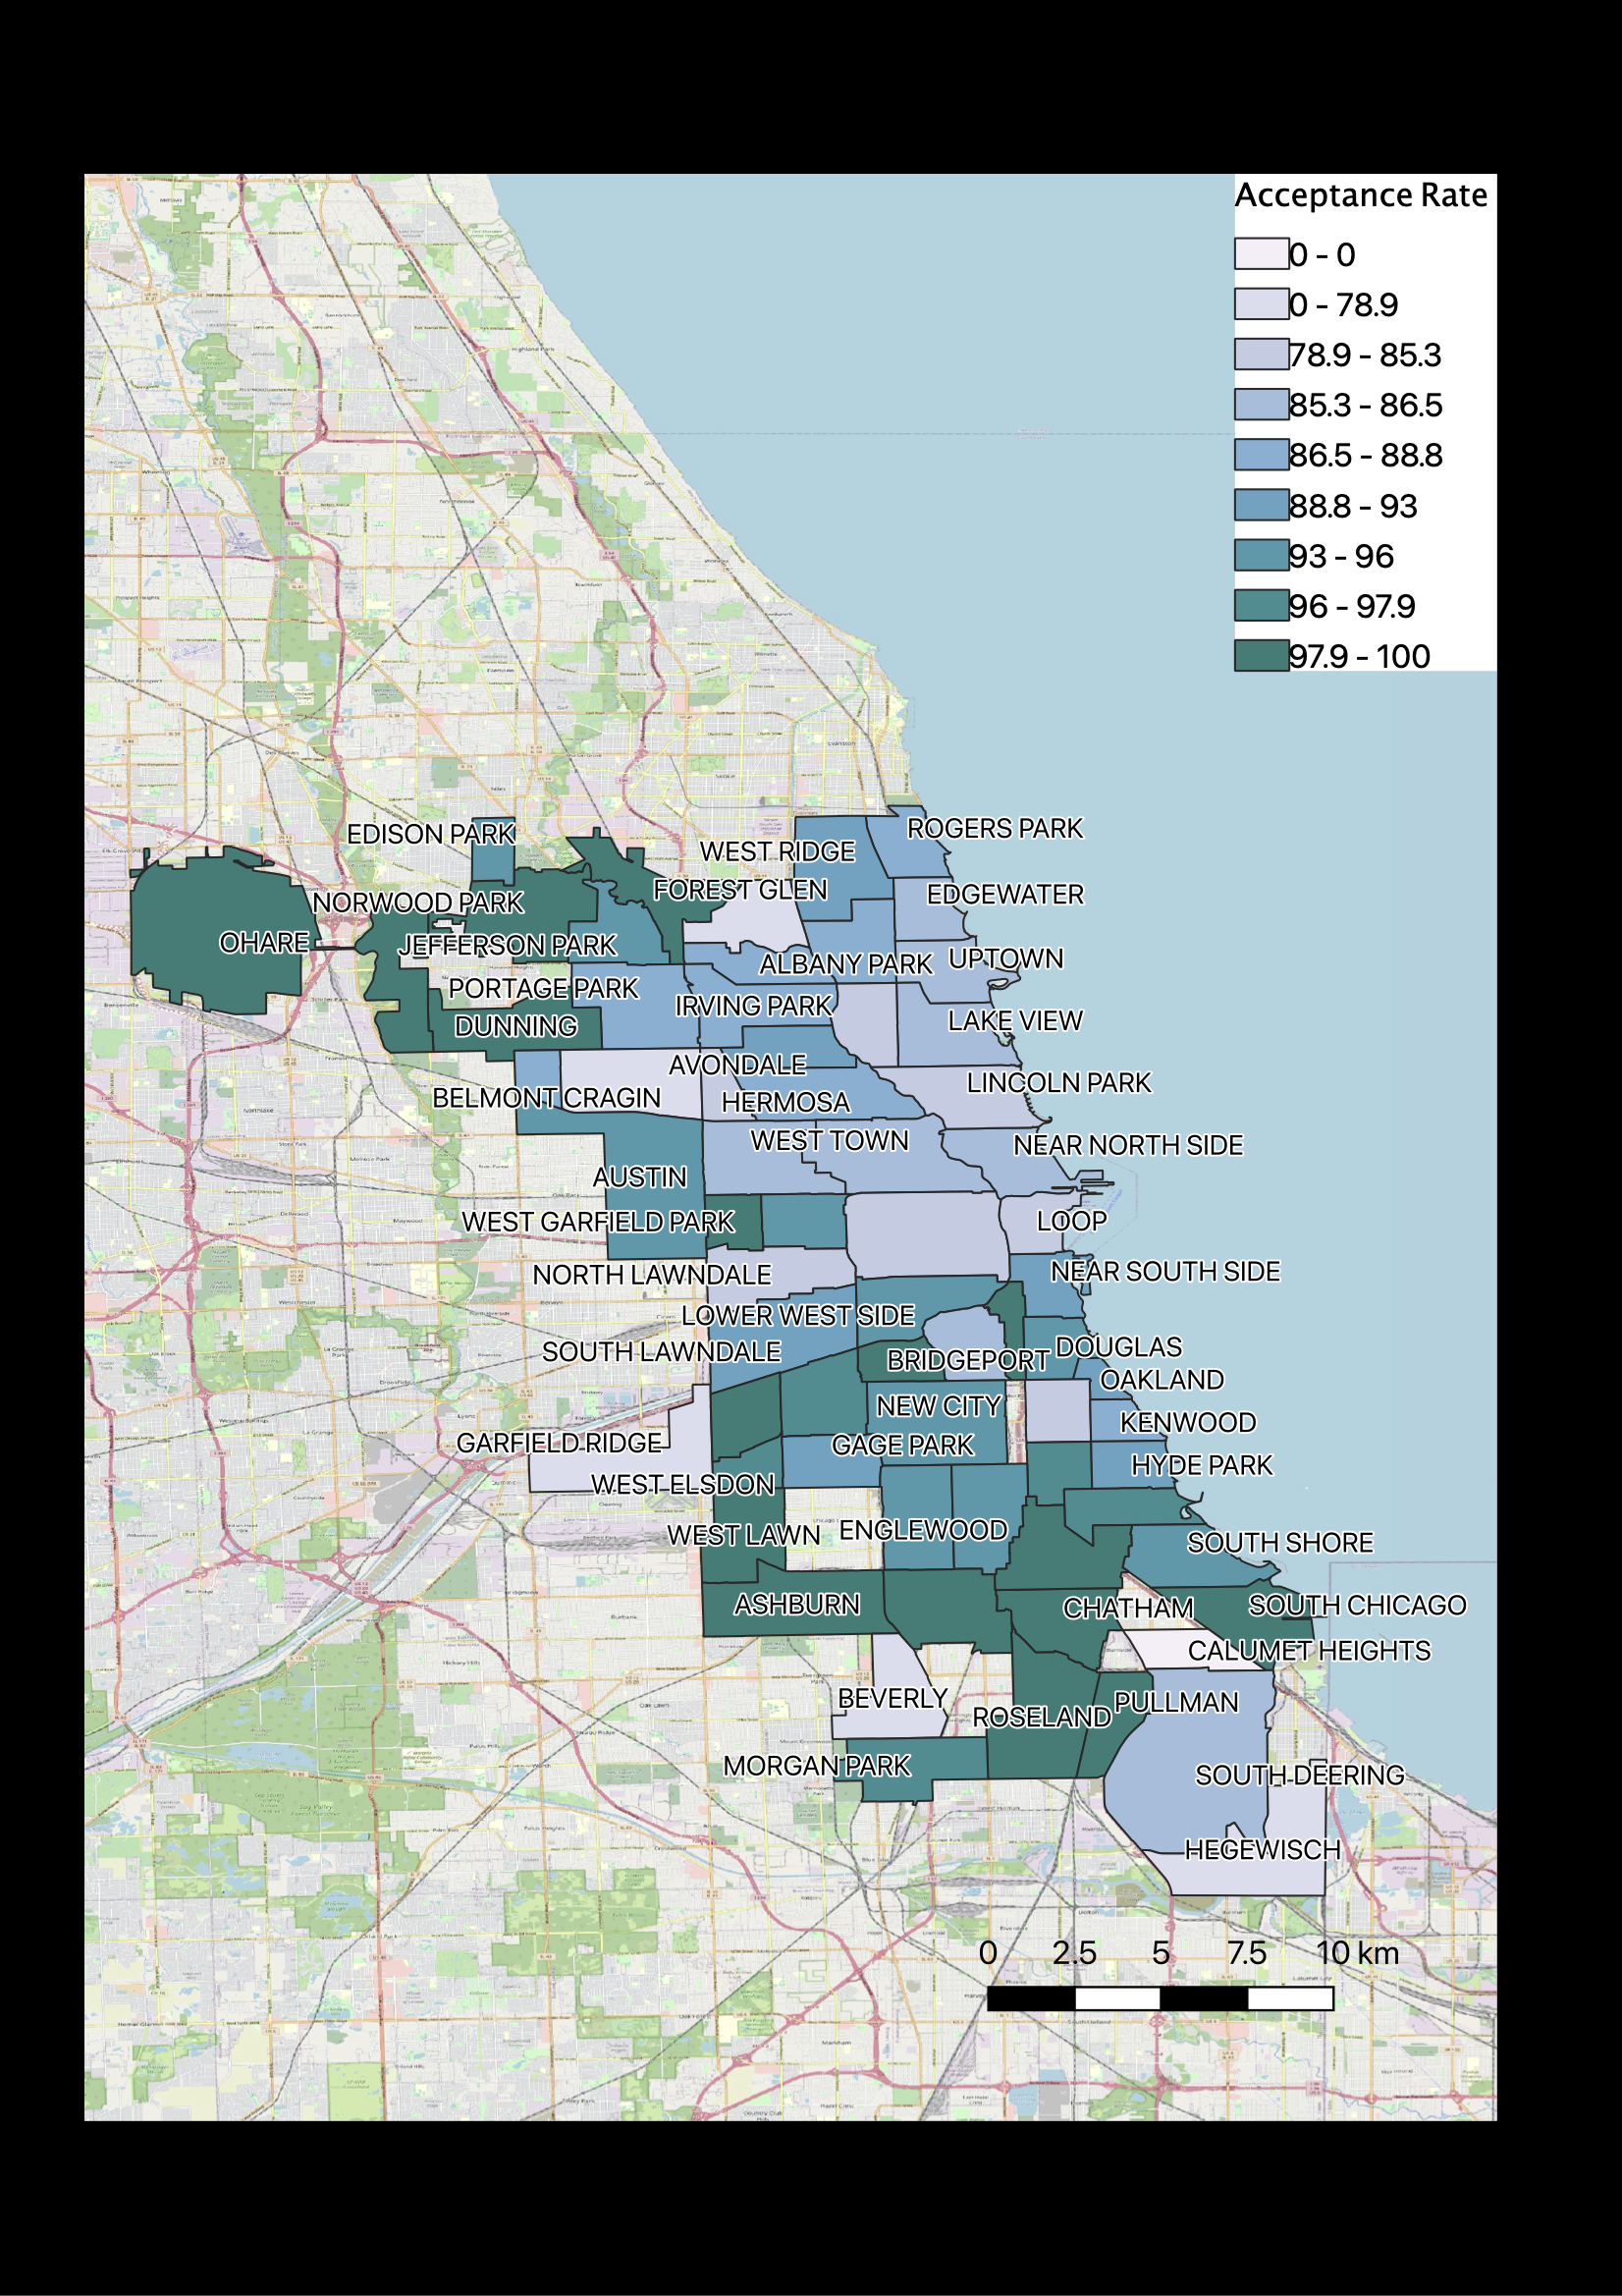
\includegraphics[width=7cm]{Acceptance Rate.png}
   \caption{Tasa de aceptación en Airbnb (\%)}
    \label{fig:my_label}
\end{figure}

\begin{figure}[!h]
    \centering
    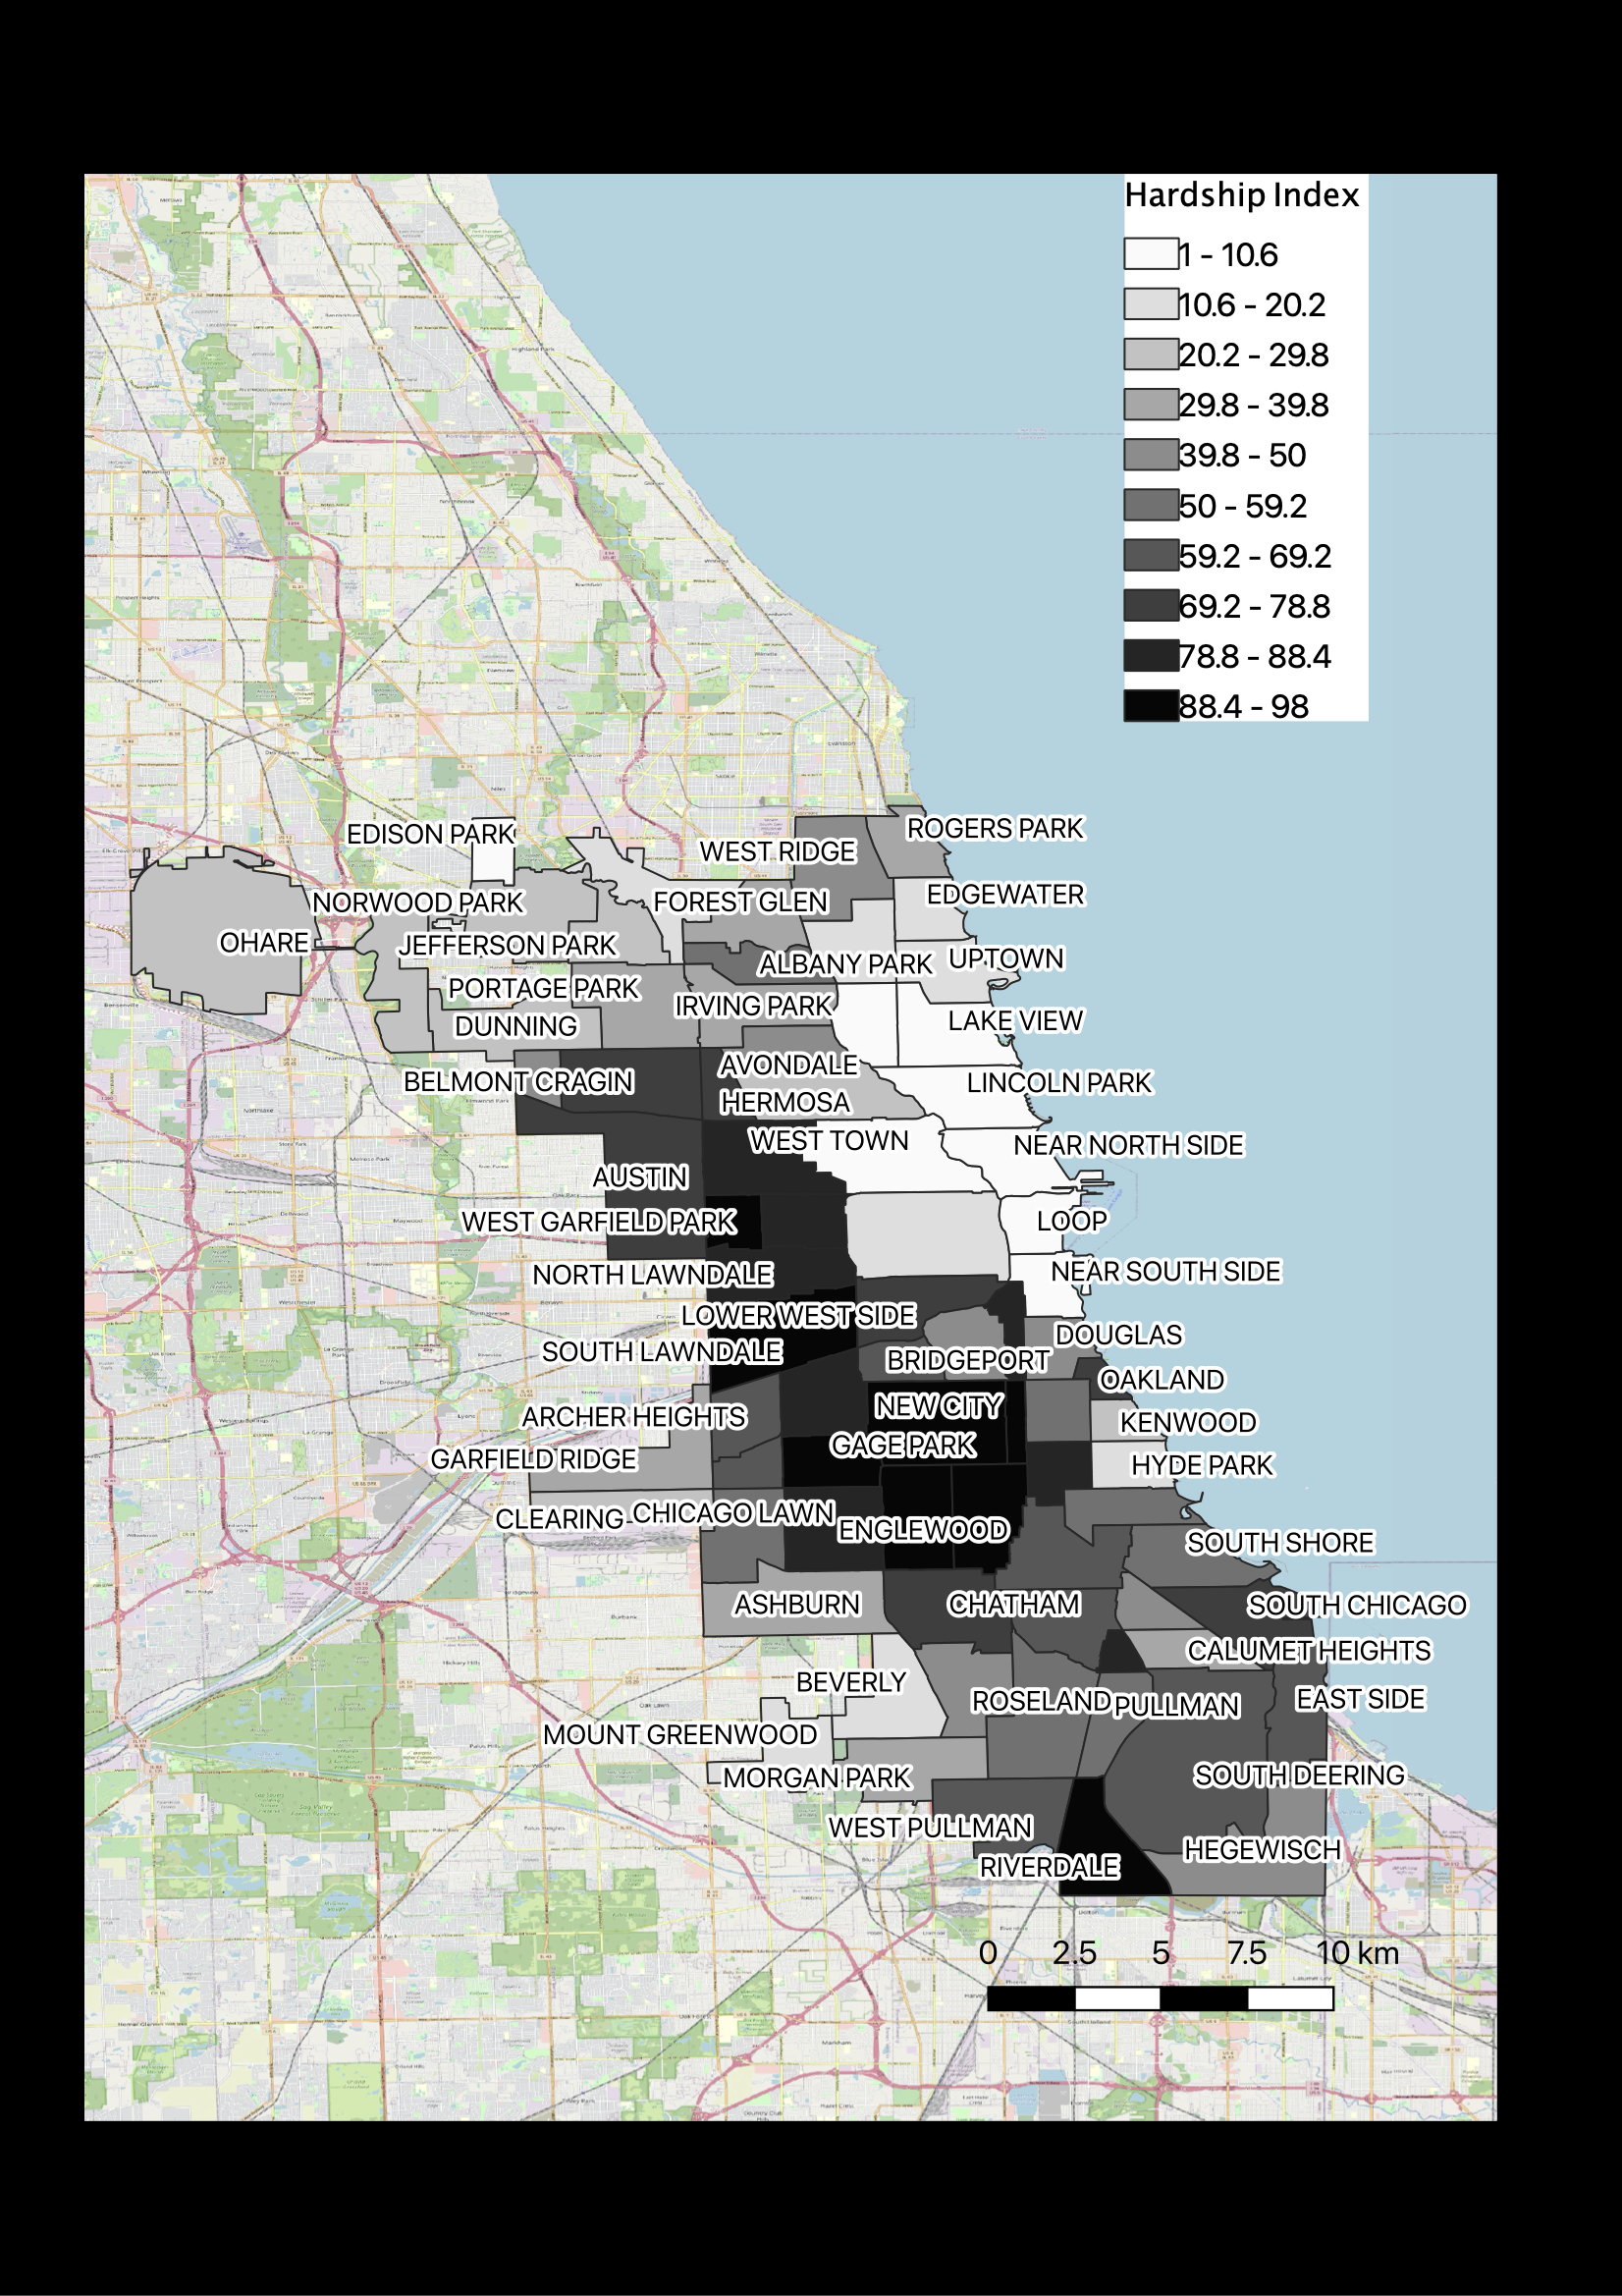
\includegraphics[width=7cm]{Hardship Index.png}
   \caption{Indice de Hardship}
    \label{fig:my_label}
\end{figure}

Por otra parte, hemos incluido tres gráficos que nos permiten describir en mayor medida las comunidades más atrayentes para el servicio de hospedaje. Primero, empleamos un gráfico de dispersión para ver la relación entre el ingreso per-cápita promedio de las comunidades y el índice de Hardship y encontramos que estos indicadores se corresponden, es decir, en las zonas con menor índice de Hardship existe mayor ingreso per-cápita promedio. Segundo, usamos un gráfico de histograma para observar la distribución de la tasa de criminalidad entre las comunidades. Finalmente, empleamos un gráfico de dispersión entre la calificación promedio de los host de Airbnb y la tasa de pobreza, se espera que las zonas con mayores niveles de pobreza carezcan de ciertos servicios e infraestructura pública, lo cual podría repercutir en una calificación desfavorable para los host.

\begin{figure}[!h]
    \centering
    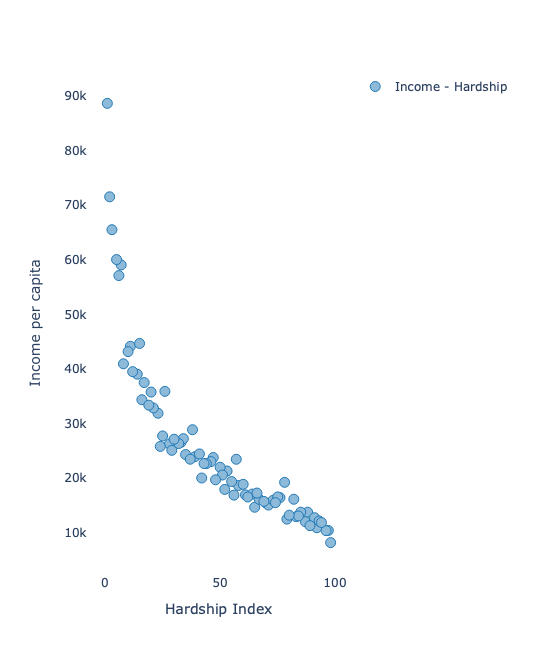
\includegraphics[width=7cm]{Part1 graph4.png}
   \caption{Relación entre ingreso per-capita e índice Hardship}
    \label{fig:my_label}
\end{figure}

\begin{figure}[!h]
    \centering
    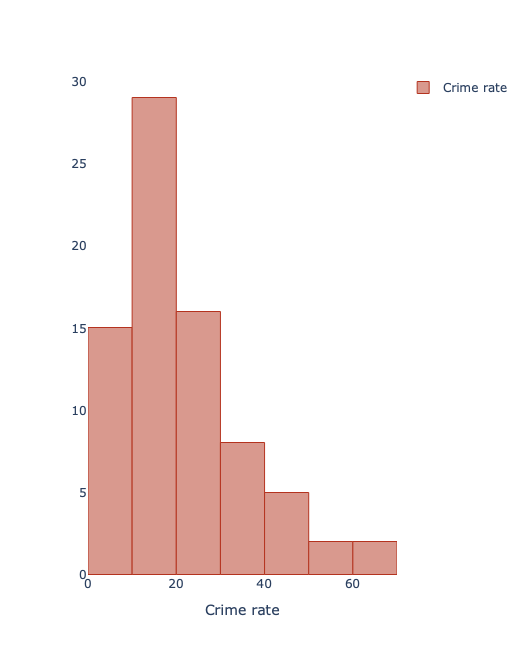
\includegraphics[width=7cm]{Part1 graph5.png}
   \caption{Distribución de tasa de crimen}
    \label{fig:my_label}
\end{figure}

\begin{figure}[!h]
    \centering
    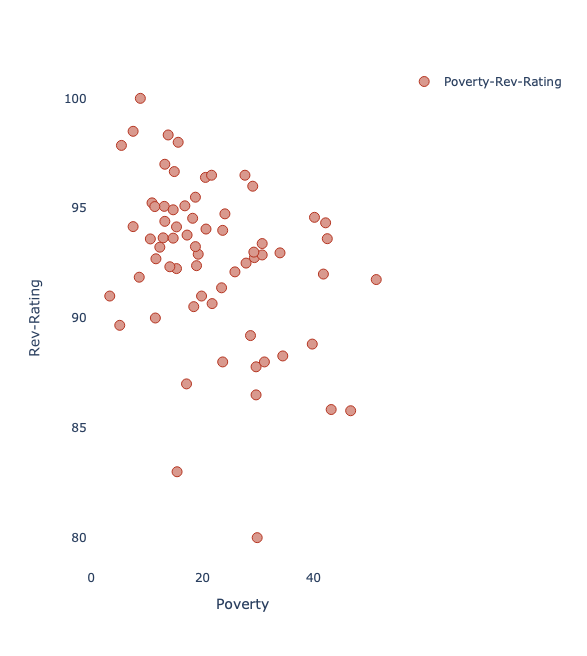
\includegraphics[width=7cm]{Part1 graph6.png}
   \caption{Relación entre calificación del host y tasa de pobreza}
    \label{fig:my_label}
\end{figure}

\clearpage
\section*{Parte 2 - Datos de Buenos Aires}

En la segunda parte del trabajo, empleamos datos de Buenos Aires correspondientes al censo del 2010. Calculamos la tasa de desempleo y la prevalencia de hogares que tienen al menos una NBI y empleamos mapas coropléticos para conocer la variabilidad de estos indicadores entre las comunidades de Buenos Aires. Respecto a la tasa de empleabilidad, encontramos que el desempleo promedio varía entre 1.5 y 5.6\%. Asimismo, encontramos que las mayores tasas de desempleo se concentran en la zona capital de la ciudad. Existen distintos mecanismos que podrían explicar por qué las zonas más cercanas a la capital muestran, en promedio, mayores niveles de desempleo. En primero lugar, al ser zonas más urbanas y con mayor concentración de personas, es posible que la disponibilidad de empleos que requieren estas zonas sea menor a la proporción de personas que las habitan. Por otro lado, estas zonas concentran a la mayor cantidad de personas que se encuentran en etapa de formación superior y al ser actividades que ocupan la mayor parte del tiempo, los imposibilita a participar activamente del mercado laboral.\\ 
Respecto a la prevalencia de hogares con al menos una NBI, encontramos varían desde 1 a 18.4\% entre las comunidades de Buenos Aires. Encontramos también que las zonas más cercanas a la capital son las que muestran mayor prevalencia de hogares con al menos una NBI y a su vez las comunidades de Villarino y Patagones también muestran alta prevalencia en este indicador. Las dinámicas que explican esta situación podrían ser similares a las de la tasa de desempleo. 

\begin{figure}[!h]
    \centering
    \subfigure[]{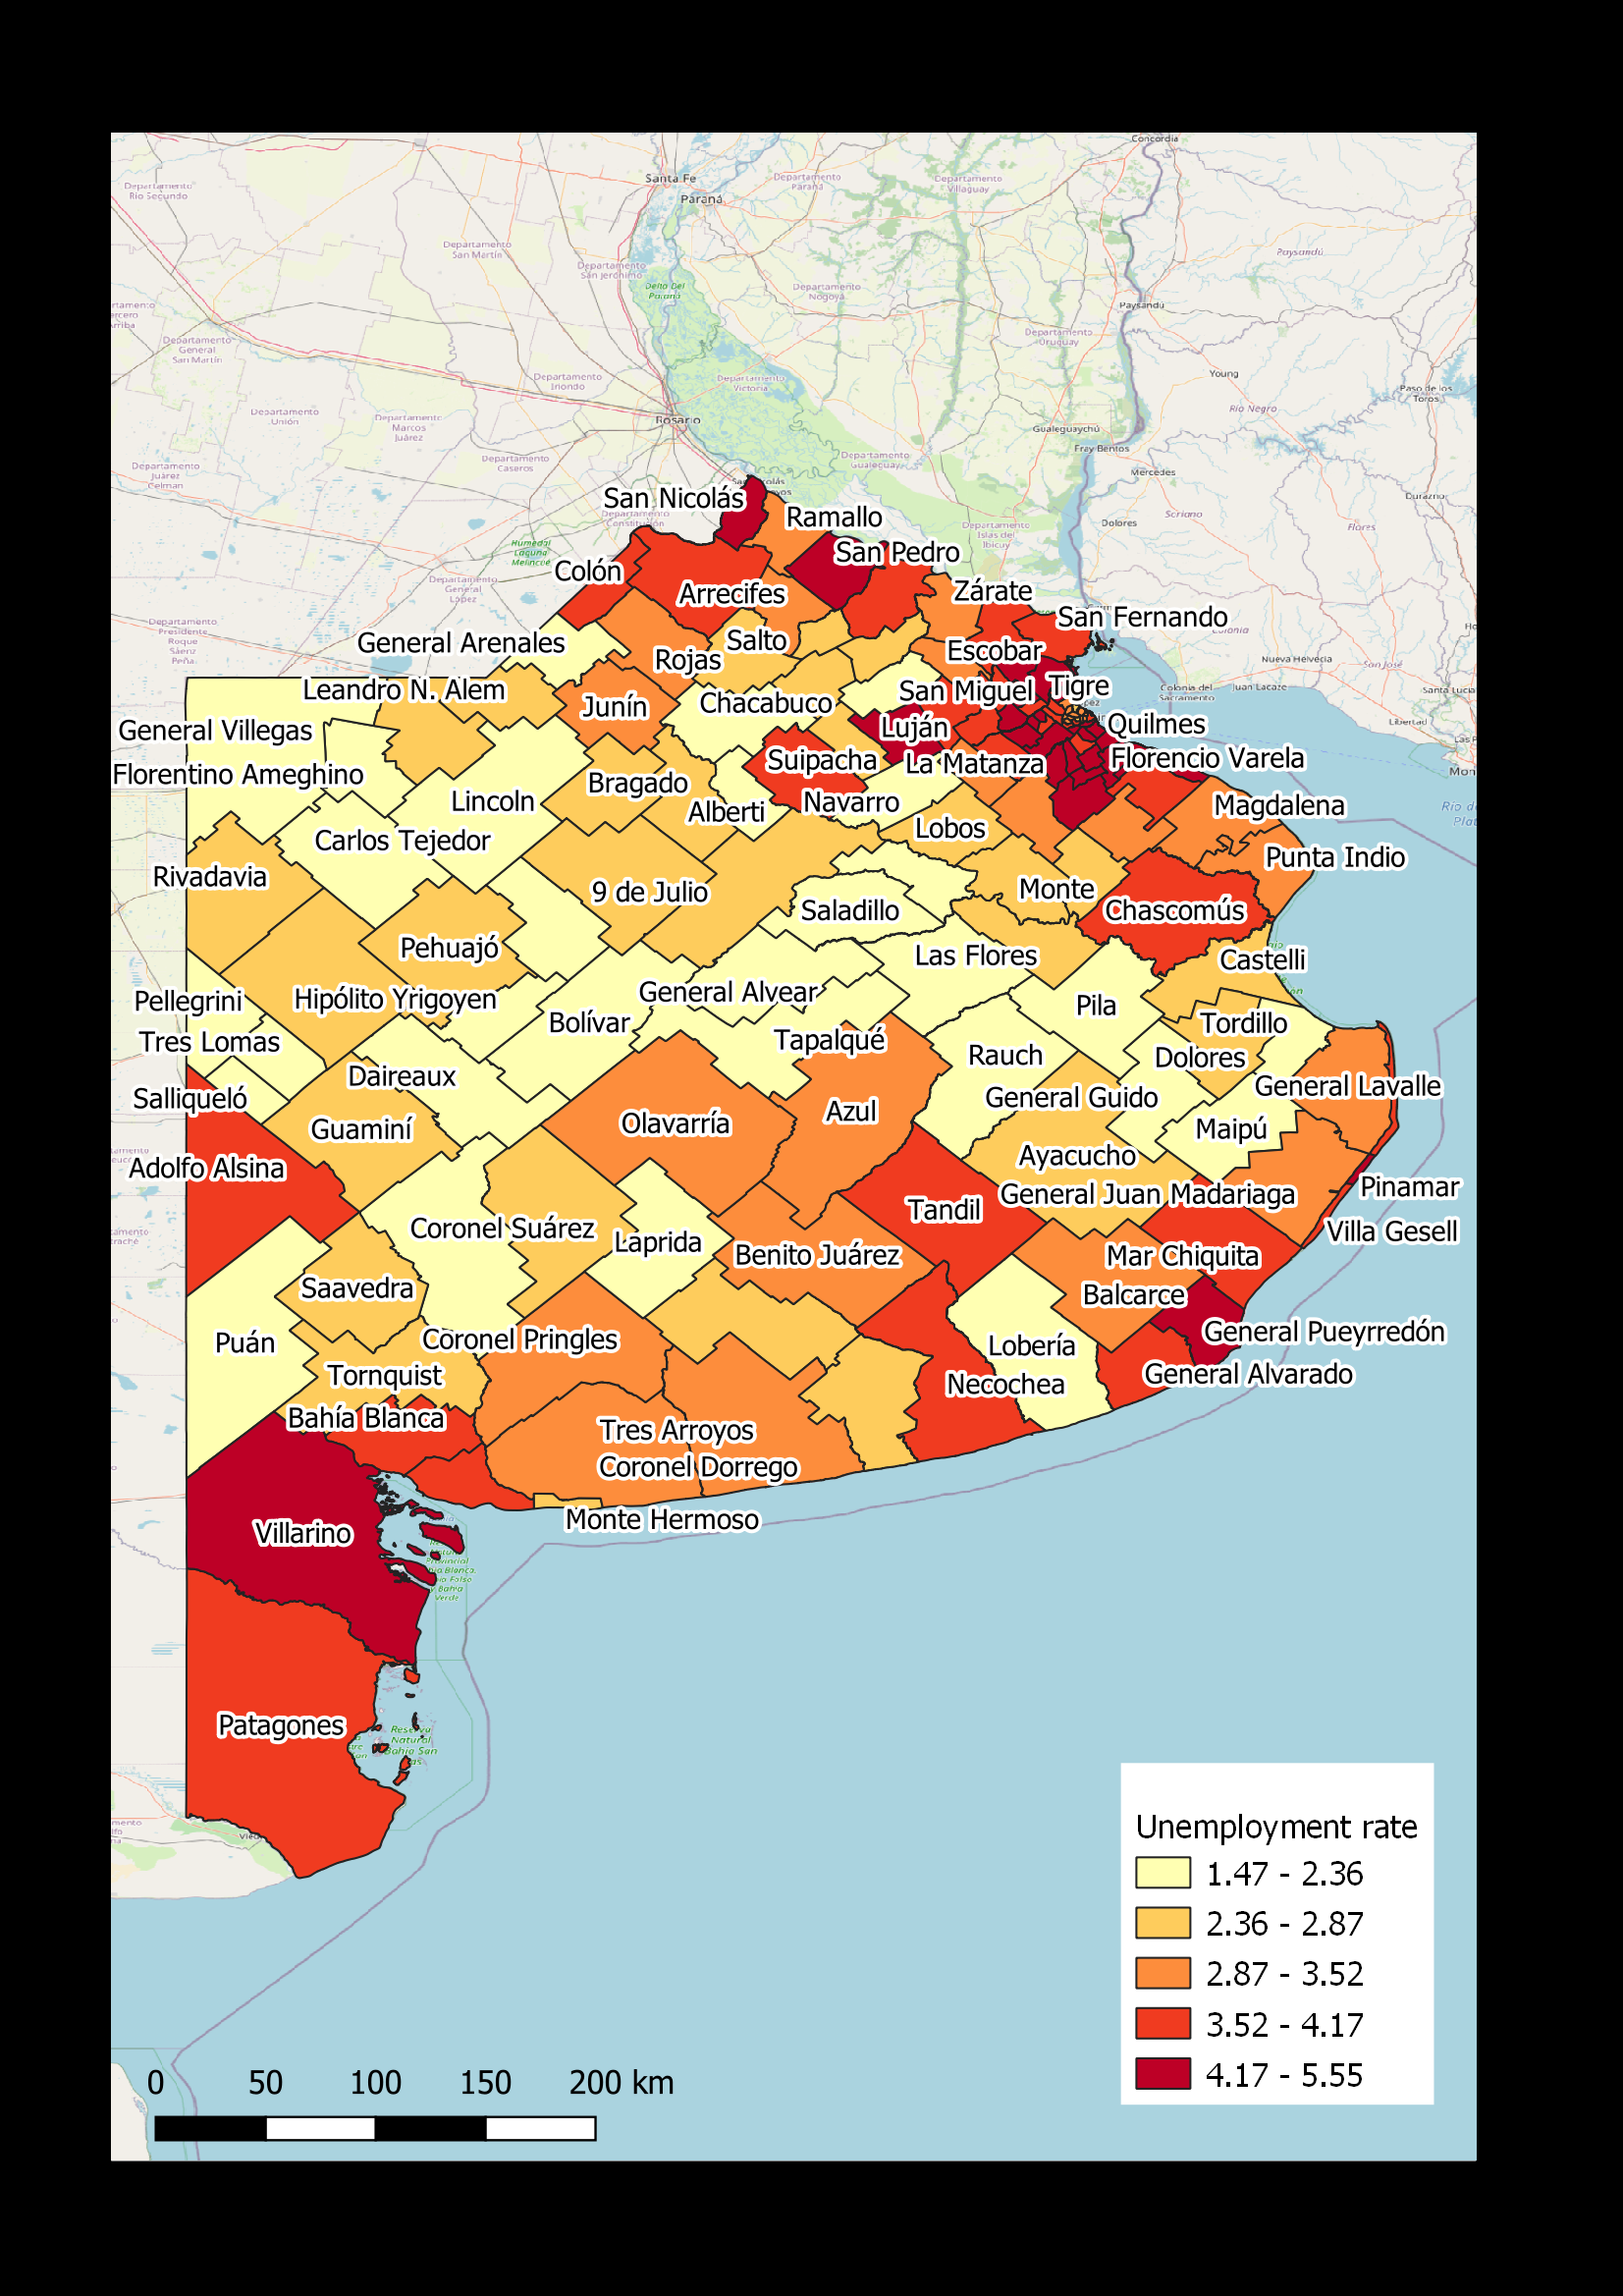
\includegraphics[width=7cm]{Part2 graph1.png}}
    \subfigure[]{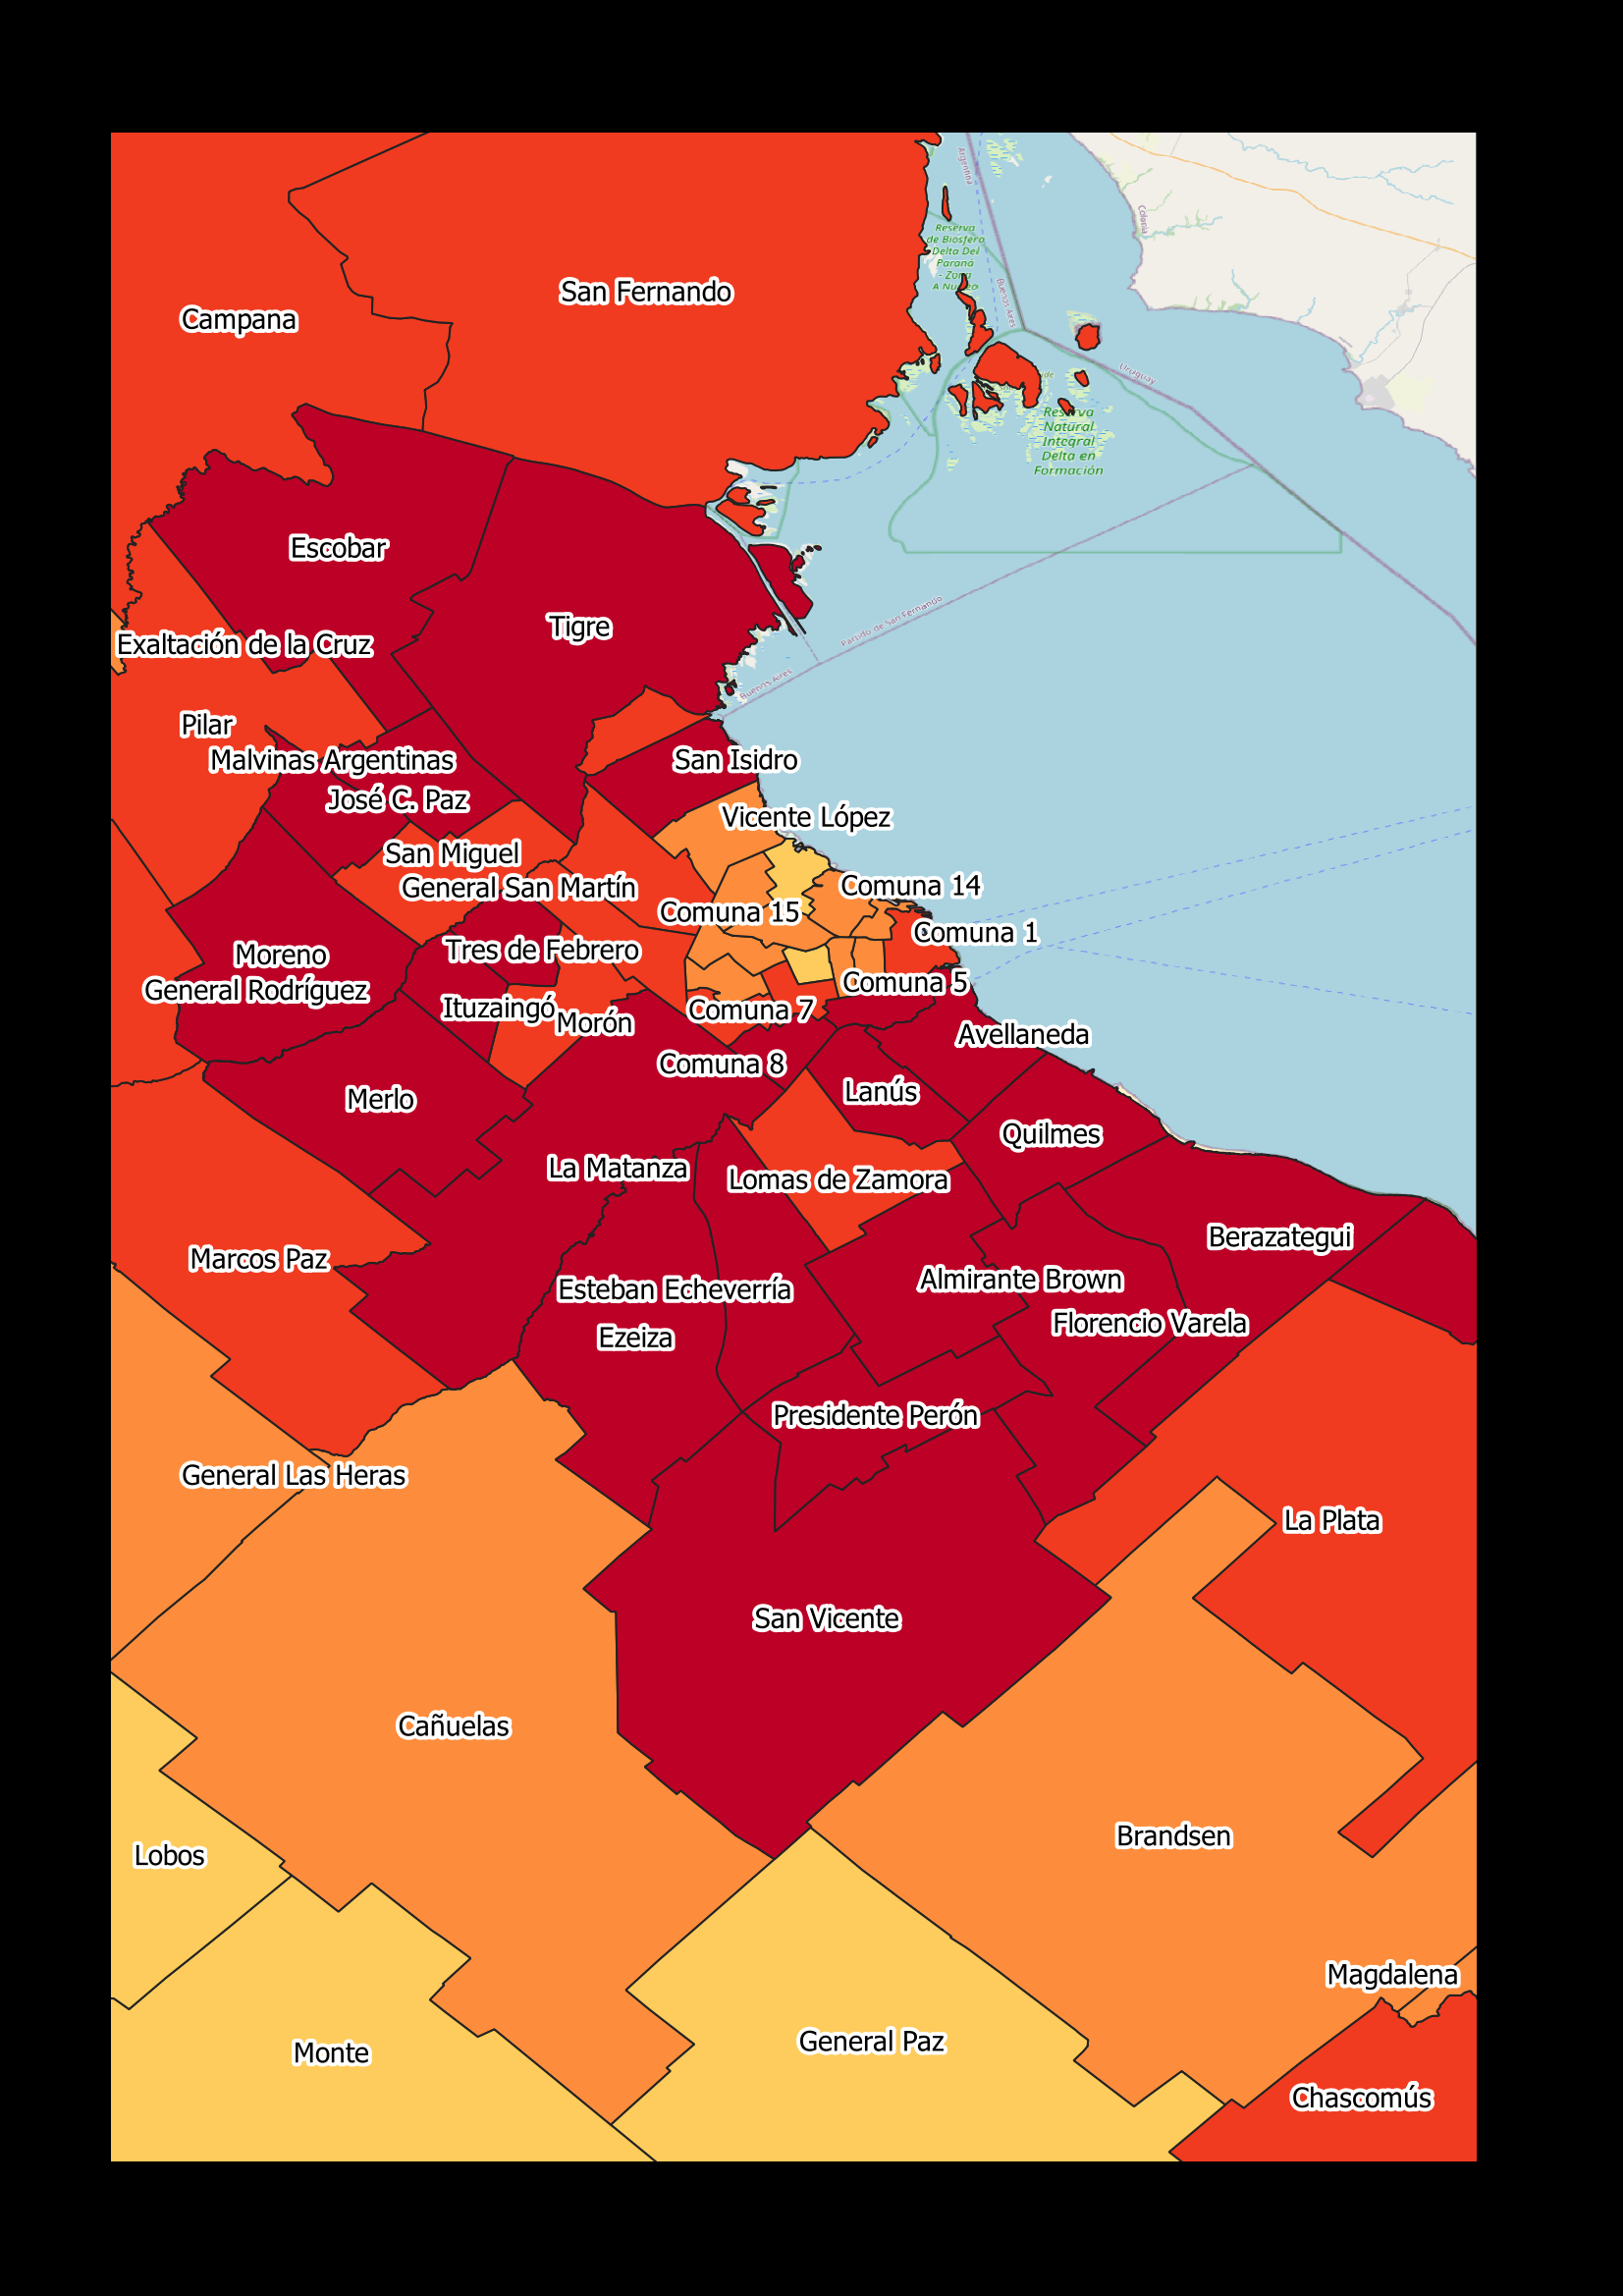
\includegraphics[width=7cm]{Part2 graph2.png}}
    \caption{Tasa de desempleo (\%)}
    \label{fig:my_label}
\end{figure}

\begin{figure}[!h]
    \centering
    \subfigure[]{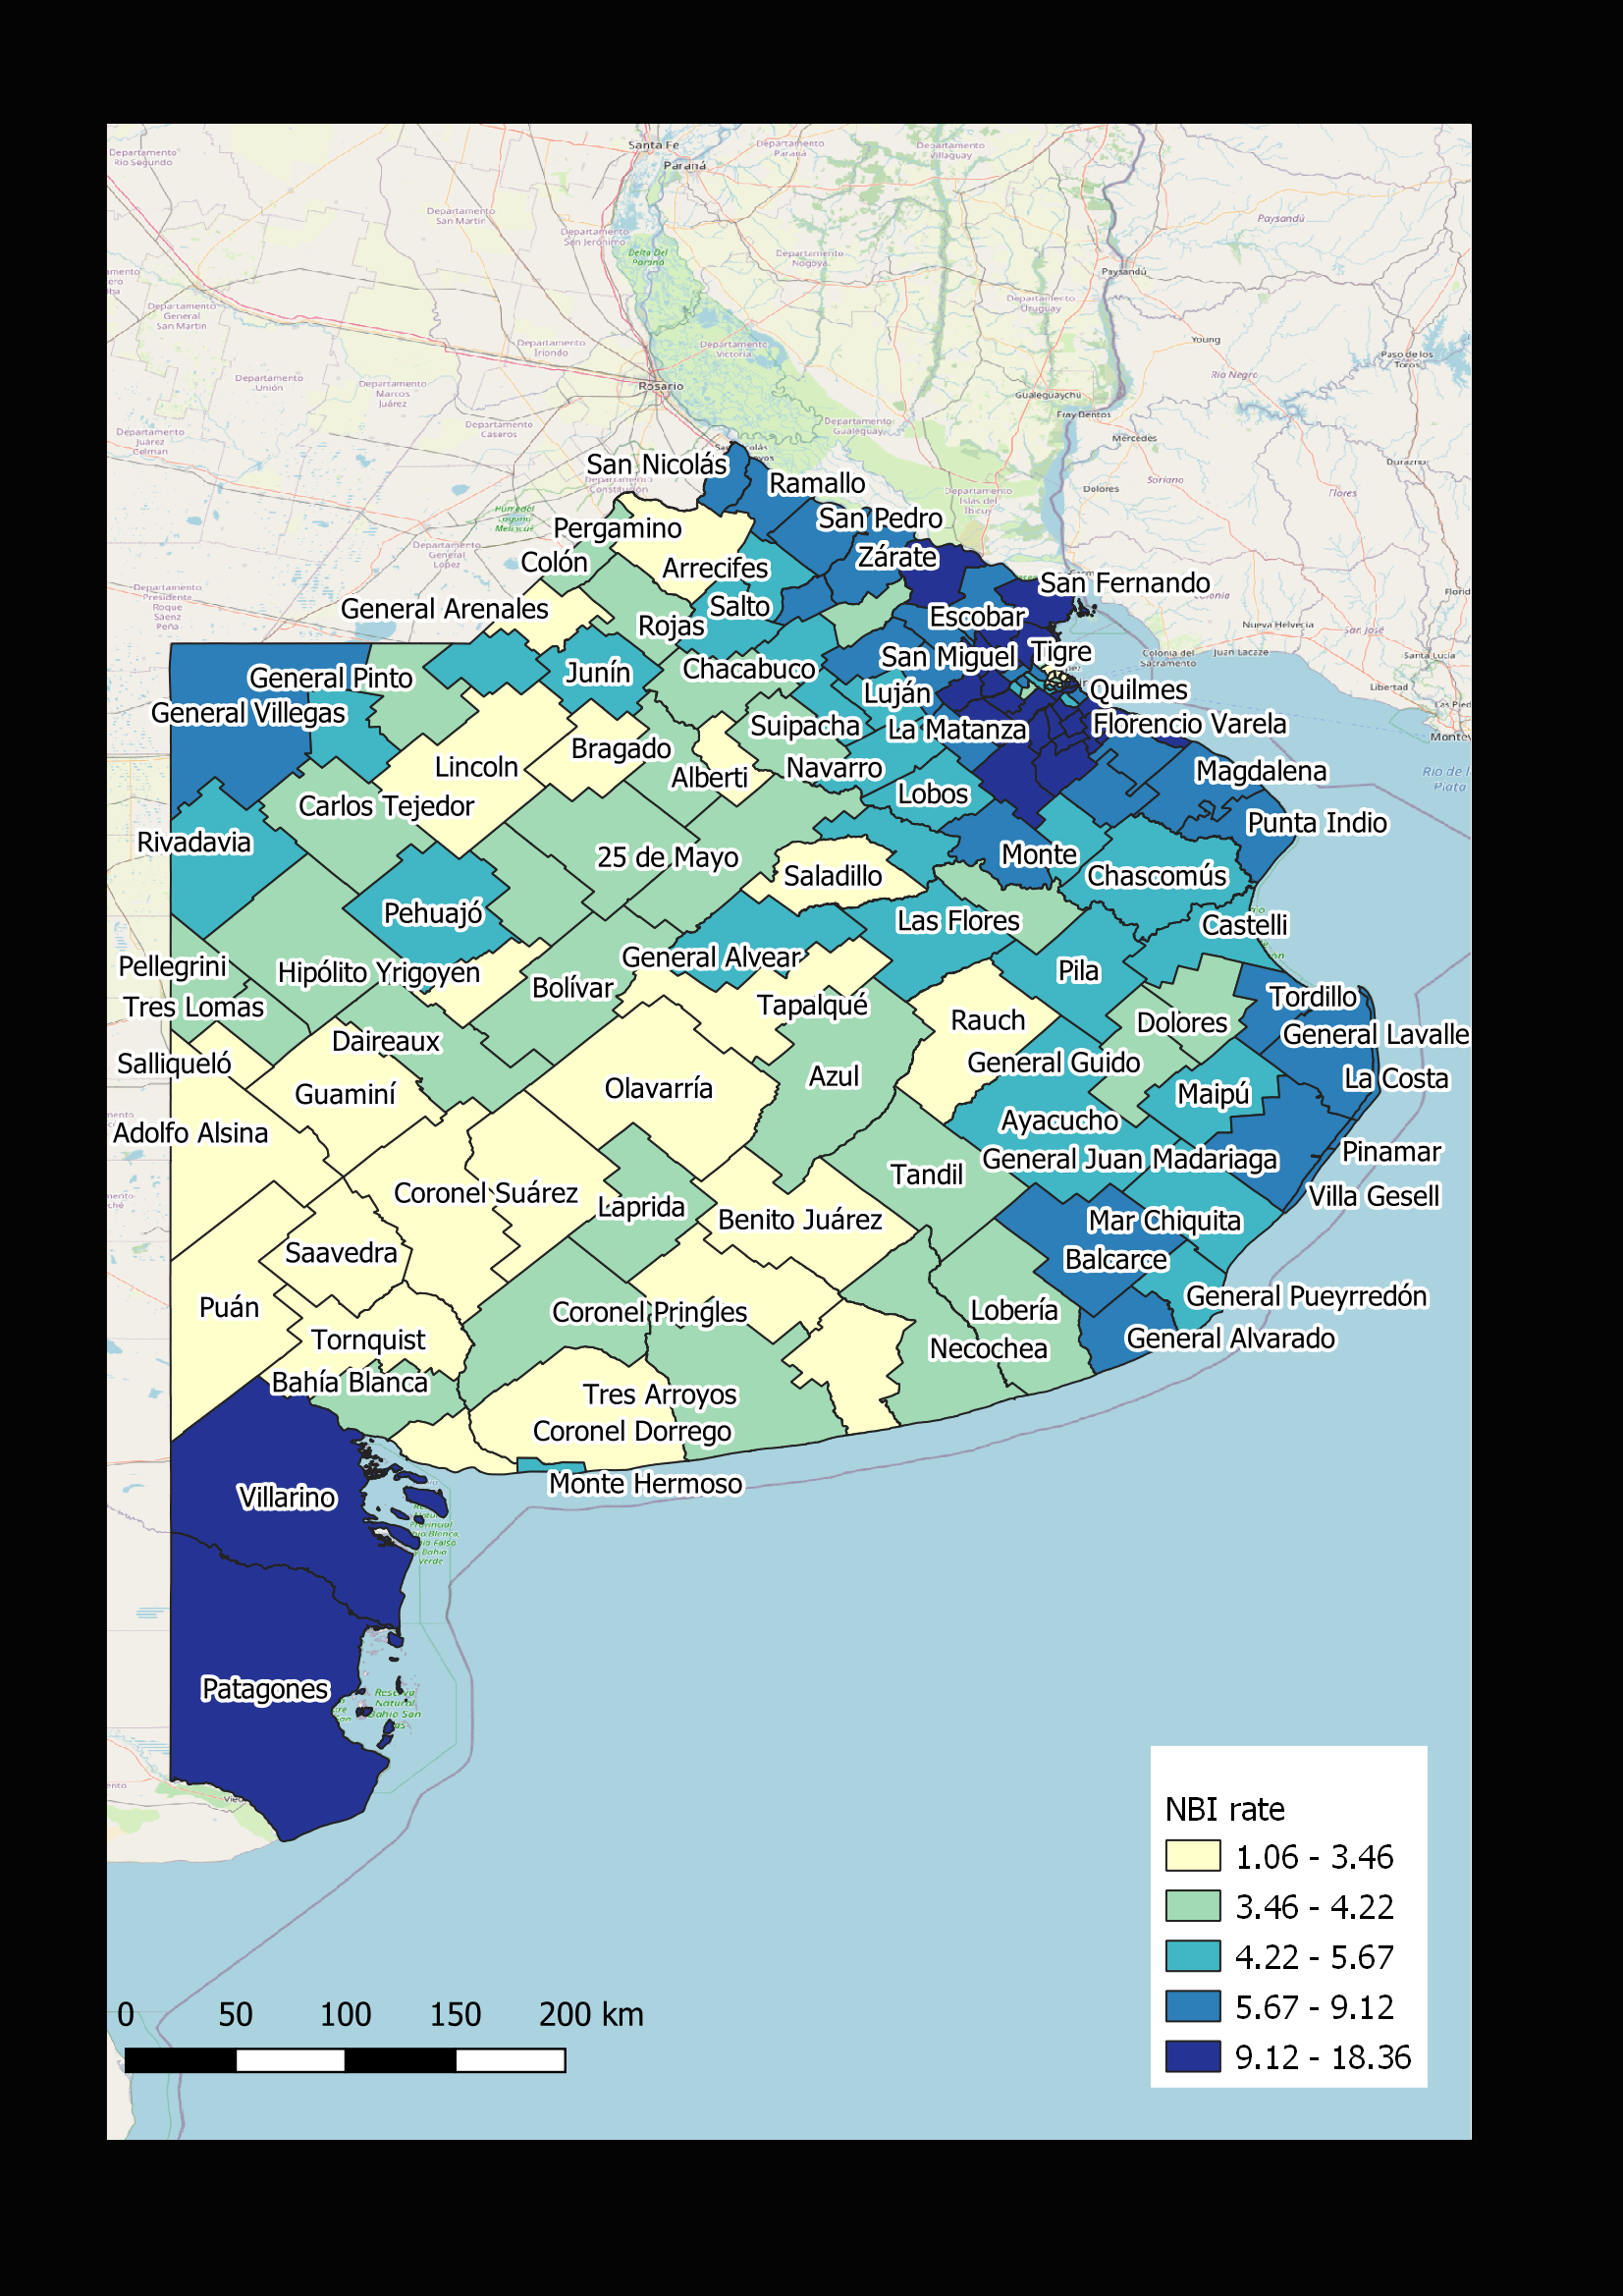
\includegraphics[width=7cm]{Part2 graph3.png}}
    \subfigure[]{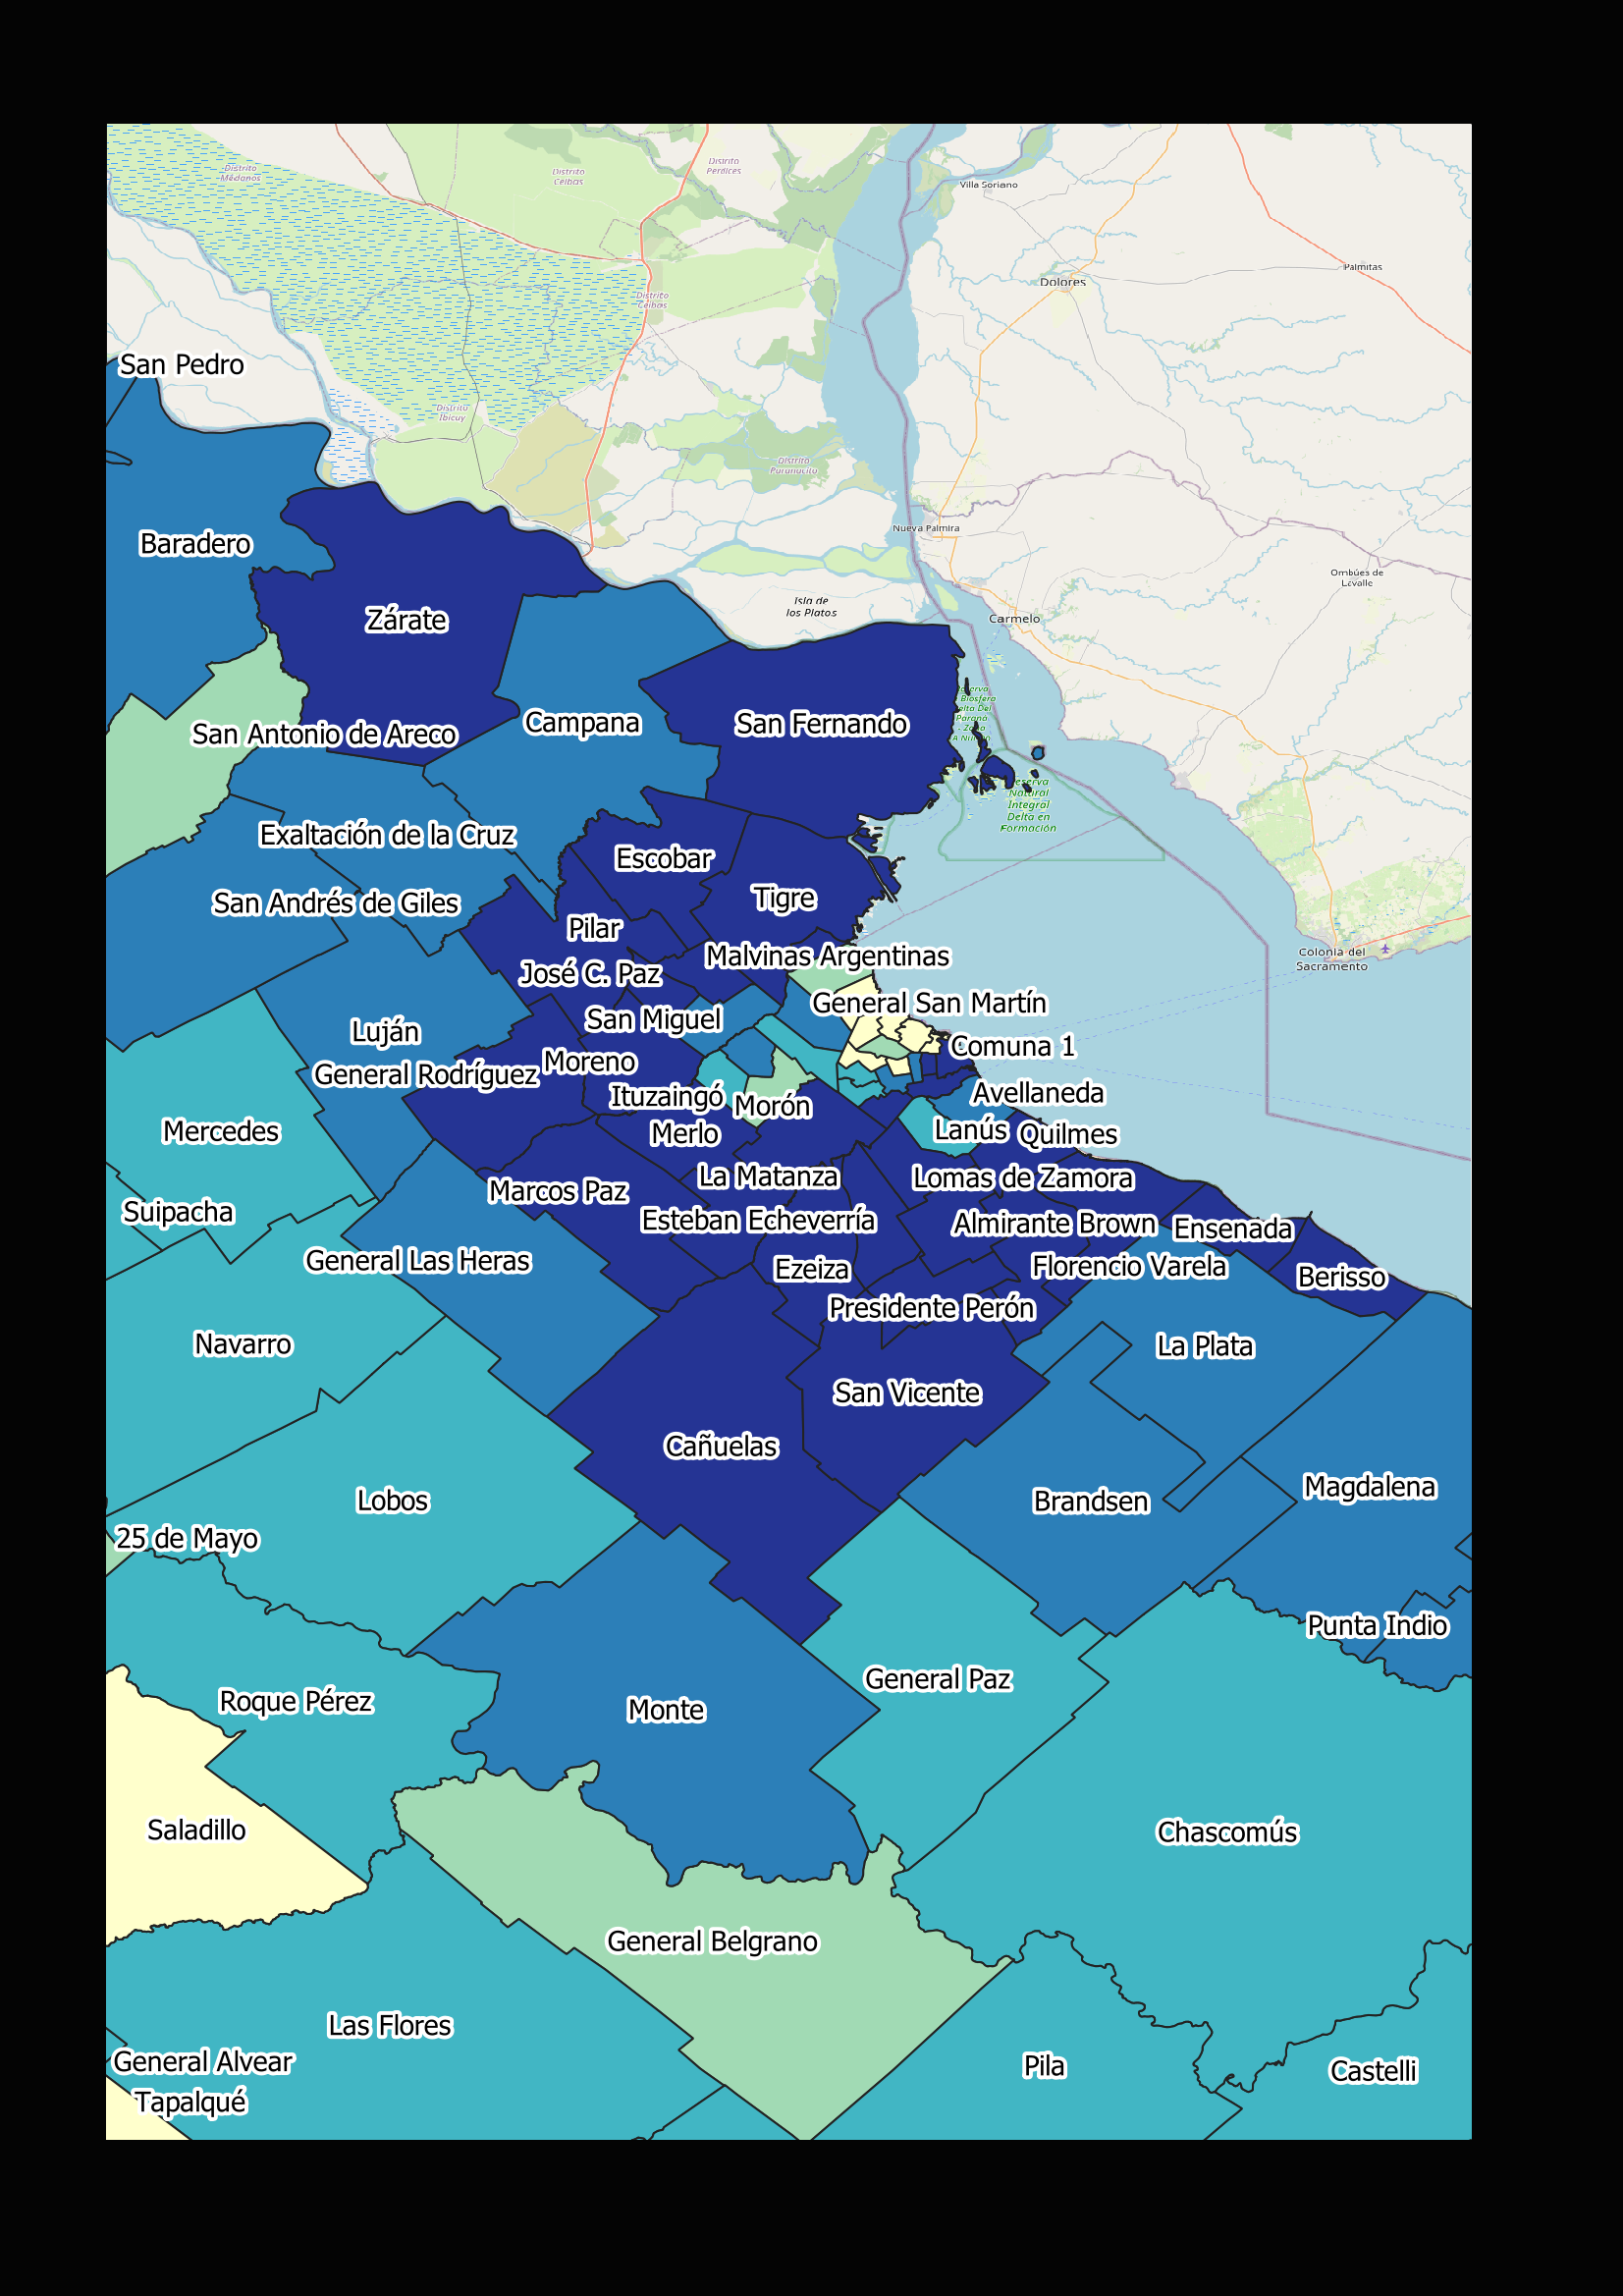
\includegraphics[width=7cm]{Part2 graph4.png}}
    \caption{Hogares que padecen de al menos una NBI (\%)}
    \label{fig:my_label}
\end{figure}



\end{document}
